\chapter{Requirements, Methodology, and Project Management}\label{chap:requirements}
\begin{spacing}{1.2}
\minitoc
\thispagestyle{MyStyle}
\end{spacing}
\newpage

\section*{INTRODUCTION}
\addcontentsline{toc}{section}{INTRODUCTION}
Chapter~\ref{chap:context} established the empirical audit findings and the resulting strategic reorientation; Chapter~\ref{chap:soa} positioned the proposed platform relative to existing technological paradigms. This chapter formalizes the engineering framework that structures the project: the stakeholders, system actors, and access control models; the functional and non-functional requirements derived from the audit; the systemic use cases and activity flows; and the agile methodology adopted to mitigate the constraints of a single-developer environment.

\section{Stakeholders, Actors, and Access Assumptions}\label{sec:stakeholders_actors}
The platform's ecosystem comprises two distinct entities: \textit{stakeholders}, whose strategic expectations define the project's criteria for success, and \textit{actors}, representing the functional roles interacting with the system via its user interfaces, APIs, or the conversational layer.

\subsection{Project Stakeholders}
Four primary stakeholders govern this project: the academic supervisor at ENET'COM, the professional supervisor at \hostCompany, the technical and executive leadership at \clientCompany, and the academic evaluation jury.

\subsection{System Actors}
The platform's interaction model defines five primary actors: three are operational within the current scope, while two are reserved for future systemic extensions. Conversational interactions via the RFQ Copilot are not modeled as an independent actor; rather, the copilot acts as a cross-cutting capability utilized by the business actors, with its access scope strictly bound to the authenticated user's privileges. Table~\ref{tab:actors} details this actor catalog.

\begin{table}[H]
\centering
\renewcommand{\arraystretch}{1.4}
\begin{tabularx}{\textwidth}{|p{2.9cm}|>{\RaggedRight\arraybackslash}X|p{1.8cm}|}
\hline
\rowcolor{lightgray}
\textbf{Actor} & \textbf{Role and Responsibilities} & \textbf{Status} \\ \hline
Estimation Manager & Exercises operational governance over the RFQ lifecycle: intake, feasibility assessment, classification, workflow orchestration, stage supervision, and final bid approval. This role mirrors the orchestration function observed within GHI's estimation department. & Current \\ \hline
Estimator & Executes granular cost estimation tasks on assigned RFQs: populates the estimation workbook, associates technical artifacts and notes to relevant lifecycle stages, and advances the RFQ through the formal estimation phase. & Current \\ \hline
Executive & Accesses portfolio-level Key Performance Indicators (KPIs) and strategic decision-support summaries via analytical endpoints and dashboards, without executing operational mutations on individual RFQs. & Current \\ \hline
Departmental User & A generalized actor representing the Engineering, Production, Quality, and Procurement functions identified during the audit (Chapter~\ref{chap:context}). Each provides stage-specific inputs and resolves departmental blockers. & Future \\ \hline
Administrator & Administers workflow templates and identity management policies, contingent upon the deployment of a dedicated Identity and Access Management (IAM) service. & Future \\ \hline
\end{tabularx}
\caption{System actors of Itqan with their responsibilities and implementation status}
\label{tab:actors}
\end{table}

\subsection{Permission Model and IAM Integration}
Each actor is bound by a strict permission scope defining RFQ visibility, permitted lifecycle mutations, and authorized analytical surfaces. Table~\ref{tab:permissions} summarizes the target permission model for the active actors. The future actors will inherit expanded permissions upon the delivery of the dedicated identity service.

\begin{table}[H]
\centering
\renewcommand{\arraystretch}{1.3}
\scriptsize
\begin{tabularx}{\textwidth}{|p{2.5cm}|>{\RaggedRight\arraybackslash}X|>{\RaggedRight\arraybackslash}X|>{\RaggedRight\arraybackslash}X|}
\hline
\rowcolor{lightgray}
\textbf{Actor} & \textbf{Lifecycle Operations} & \textbf{Analytics Surface} & \textbf{Copilot Scope} \\ \hline
Estimation Manager & Full read and write privileges across the departmental portfolio; holds authority for classification, approval, and stage supervision. & Comprehensive portfolio analytics. & Portfolio mode and RFQ-bound mode across all departmental RFQs. \\ \hline
Estimator & Read and write privileges strictly limited to assigned RFQs; authorized to advance assigned RFQs through estimation stages. & Read-only access to personal pipeline metrics. & RFQ-bound mode on assigned RFQs; portfolio mode scoped exclusively to assigned RFQs. \\ \hline
Executive & Read-only access to portfolio aggregates; prohibited from executing state mutations on individual RFQs. & Comprehensive portfolio analytics and strategic summaries. & Portfolio mode only. \\ \hline
\end{tabularx}
\caption{Target permission model for currently exercised actors}
\label{tab:permissions}
\end{table}

In the current implementation, this permission model is enforced via \textit{actor-context propagation}: every inbound request carries an actor context in the current prototype, which the manager service uses to scope data retrieval and protect state-mutating operations. The copilot inherits this exact scope rather than maintaining an independent authorization matrix, as every evidence retrieval request is routed through the manager service's scoped endpoints (FR-COP-06, NFR-SEC-02). A dedicated \textit{Identity and Access Management (IAM) service} is architecturally reserved as a future integration point within the manager (Authorization-header forwarding and an identity-resolution connector, with token validation delegated to the future service). Comprehensive cross-tenant isolation and granular role-based access control (RBAC) are deferred to this future IAM service (NFR-SEC-01, NFR-SEC-04).


\section{Functional Requirements}\label{sec:functional_requirements}
The functional requirements delineate the mandatory operational capabilities provided to the actors defined in Section~\ref{sec:stakeholders_actors}. These requirements are derived directly from the operational constraints documented in Chapter~\ref{chap:context}; each constraint informs one or more specific requirements. They are categorized by system module and assigned unique identifiers for traceability against the validation evidence in Chapter~\ref{chap:validation}.

The twenty-five functional requirements are distributed across the four platform modules and cross-cutting domains. Eight \textbf{Manager-service} requirements (FR-MGR-01 to FR-MGR-08) govern RFQ registration with classification metadata, workflow-driven stage instantiation, three-gate stage progression (mandatory-field, blocker, transition-validity), artifact association with append-only note semantics, manual and rule-based reminder automation, analytical aggregations (status distributions, win-rates, client-specific metrics), lifecycle traceability via non-destructive update semantics, and cascading soft-deletion for subtasks. Eight \textbf{Copilot-service} requirements (FR-COP-01 to FR-COP-08) define evidence-grounded natural-language generation, dual contextual entry points (portfolio vs. RFQ-bound), deterministic turn classification, path-authorized evidence retrieval (currently bounded to manager state, extensible to intelligence artifacts), structured refusal mechanisms for out-of-scope queries, manager-mediated access enforcement, bounded working-memory management, and strict pre-delivery response verification. Four \textbf{Intelligence-service} requirements (FR-INT-01 to FR-INT-04) dictate deterministic parsing of MR-packages against canonical layouts, estimation-workbook parsing against the GHI template (\textit{General}, \textit{Bid~S}, \textit{Top Sheet} anchor set), intelligence briefing generation, and structured anomaly reporting over silent error suppression. Three \textbf{User-Interface} requirements (FR-UI-01 to FR-UI-03) specify the portfolio dashboard, detailed RFQ views, and role-aware executive indicator surfaces. Two \textbf{Cross-cutting} requirements (FR-X-01, FR-X-02) mandate independent backend containerization and standardized health and observability endpoints.

The comprehensive product backlog, detailing priority levels and implementation statuses, is documented in Appendix~\ref{app:backlog} (Table~\ref{tab:backlog}). Detailed implementation and validation coverage for each requirement are analyzed in Chapters~\ref{chap:implementation} and~\ref{chap:validation}.

\subsection{Product Backlog}
The aforementioned functional requirements are managed operationally as a 25-item prioritized product backlog (Appendix~\ref{app:backlog}). The dedicated IAM service is tracked as a deliberately deferred item outside this active backlog, as established in Chapter~\ref{chap:context}.

\section{Non-Functional Requirements}\label{sec:non_functional_requirements}
The non-functional requirements encompass standard production-grade constraints alongside specific imperatives for an LLM-based conversational layer. They are categorized into five domains: Reliability (REL), Security (SEC), AI Integrity (AI), Maintainability (MNT), and Operability (OPS). Each requirement is tagged with a Scope/Status indicator distinguishing fully implemented attributes from partial or deferred components (Table~\ref{tab:nfr}).


\begingroup
\renewcommand{\arraystretch}{1.2}
\scriptsize
\begin{longtable}{|p{2.2cm}|p{2.7cm}|>{\RaggedRight\arraybackslash}p{5.8cm}|p{2.7cm}|}
\caption{Non-functional requirements grouped by category, indicating current scope and implementation status}
\label{tab:nfr} \\
\hline
\rowcolor{lightgray}
\textbf{ID} & \textbf{Category} & \textbf{Requirement} & \textbf{Scope / Status} \\ \hline
\endfirsthead
\multicolumn{4}{l}{\textit{\tablename~\thetable\ --- continued from previous page}} \\
\hline
\rowcolor{lightgray}
\textbf{ID} & \textbf{Category} & \textbf{Requirement} & \textbf{Scope / Status} \\ \hline
\endhead
\hline
\multicolumn{4}{r}{\textit{continued on next page}} \\
\endfoot
\hline
\endlastfoot
NFR-REL-01 & Reliability & State-mutating operations on lifecycle records shall preserve traceability via timestamps and non-destructive update semantics; a dedicated audit-log surface represents a hardening direction. & Implemented; audit-log hardening direction \\ \hline
NFR-REL-02 & Reliability & The system shall fail safely during transient infrastructure anomalies, preserving persisted state and returning structured error payloads to facilitate safe re-execution. & Partial; safe-failure implemented, automatic retry deferred \\ \hline
NFR-REL-03 & Reliability & Records flagged for soft deletion shall remain accessible for auditing; no destructive deletion shall execute on critical lifecycle data. & Implemented \\ \hline
NFR-REL-04 & Reliability & State mutations and errors within the manager service shall propagate a structured correlation identifier to support distributed tracing. & Partial; manager-internal implemented, cross-service deferred \\ \hline
NFR-SEC-01 & Security & Role-Based Access Control (RBAC) shall be enforced at the service layer independently of the client. Currently exercised via actor-context headers and manager-mediated retrieval; full IAM integration is deferred. & Partial; IAM integration point built, identity service deferred \\ \hline
NFR-SEC-02 & Security & The copilot service shall explicitly not bypass manager access controls: all evidence retrieval must route through authorized manager endpoints. & Implemented \\ \hline
NFR-SEC-03 & Security & Authentication credentials and external API keys shall be strictly excluded from application logs, HTTP responses, and persistence layers. & Implemented as coding discipline; automated redaction tests deferred \\ \hline
NFR-SEC-04 & Security & Database schemas and queries shall ensure per-user data scoping; absolute cross-tenant data isolation is contingent upon the deferred IAM service. & Partial; IAM deferred \\ \hline
NFR-AI-01 & AI Integrity & The copilot shall not generate factual claims regarding RFQs, lifecycle states, or platform data unsupported by evidence retrieved during the current computational turn. & Implemented (Path~4) \\ \hline
NFR-AI-02 & AI Integrity & The copilot shall explicitly justify its responses by referencing the retrieved evidence, ensuring claim verifiability. & Implemented (Path~4) \\ \hline
NFR-AI-03 & AI Integrity & The copilot shall execute a structured refusal, rather than a probabilistic approximation, for queries outside its defined scope or lacking sufficient evidence. & Implemented \\ \hline
NFR-AI-04 & AI Integrity & Authority over operational truth, evidence selection, and access enforcement shall reside exclusively within deterministic platform components, not the language model. & Implemented \\ \hline
NFR-MNT-01 & Maintainability & Services shall expose capabilities strictly through versioned, documented API contracts; internal data structures shall remain encapsulated within service boundaries. & Implemented \\ \hline
NFR-MNT-02 & Maintainability & Backend services shall implement the BACAB layered architecture (routes, controllers, datasources, supported by translators, models, configuration, and utilities). & Implemented (backend services) \\ \hline
NFR-MNT-03 & Maintainability & Major architectural decisions shall be formalized in an Architectural Decision Record (ADR) detailing context, alternatives, and consequences. & Implemented for headline decisions (e.g., ADR-H5) \\ \hline
NFR-OPS-01 & Operability & Backend services shall be containerized and independently deployable, with externalized configuration management. & Partial; backend containerized, root composition deferred \\ \hline
NFR-OPS-02 & Operability & Backend services shall expose standardized health endpoints; readiness and metrics endpoints shall be provided where applicable. & Partial; /health implemented universally, /metrics on manager \\ \hline
NFR-OPS-03 & Operability & The manager service shall emit structured telemetry including a correlation identifier; propagating structured logging across all services is a hardening direction. & Partial; manager only, cross-service propagation deferred \\ \hline
NFR-OPS-04 & Operability & Synchronous operational endpoints shall maintain latency compatible with interactive user experiences under nominal load. & Observed during functional testing \\ \hline
\end{longtable}
\endgroup


\section{Use Cases and Activity Diagrams}\label{sec:use_cases}
This section details the behavioral architecture of Itqan: the systemic use cases through which actors interact with the platform, and the activity flow defining the core lifecycle workflow.

\subsection{System-Level Use Cases}
Eight fundamental use cases define the interaction surface of Itqan. Table~\ref{tab:use_case_matrix} presents the actor-use-case responsibility matrix, correlating actors with their authorized execution scopes.

\begin{table}[H]
\centering
\renewcommand{\arraystretch}{1.3}
\scriptsize
\begin{tabularx}{\textwidth}{|>{\RaggedRight\arraybackslash}X|c|c|c|c|c|}
\hline
\rowcolor{lightgray}
\textbf{Use Case} & \textbf{Manager} & \textbf{Estimator} & \textbf{Executive} & \textbf{Dept. User (future)} & \textbf{Admin (future)} \\ \hline
Consult RFQ Portfolio & $\checkmark$ & $\checkmark$ (scoped) & $\checkmark$ & $\checkmark$ & --- \\ \hline
Register RFQ & $\checkmark$ & --- & --- & --- & --- \\ \hline
Advance RFQ Stage & $\checkmark$ & $\checkmark$ (assigned) & --- & $\checkmark$ (own stage) & --- \\ \hline
Manage Stage Artifacts & $\checkmark$ & $\checkmark$ (assigned) & --- & $\checkmark$ (own stage) & --- \\ \hline
Configure Reminders & $\checkmark$ & $\checkmark$ (own) & --- & $\checkmark$ (own) & --- \\ \hline
Consult Pipeline Analytics & $\checkmark$ & $\checkmark$ (limited) & $\checkmark$ & --- & --- \\ \hline
Consult the RFQ Copilot & $\checkmark$ & $\checkmark$ (scoped) & $\checkmark$ (portfolio mode) & $\checkmark$ & --- \\ \hline
Manage Workflow Templates & --- & --- & --- & --- & $\checkmark$ \\ \hline
\end{tabularx}
\caption{Actor-use-case responsibility matrix indicating access scope per role}
\label{tab:use_case_matrix}
\end{table}

The use cases are formally defined as follows. \textit{Consult RFQ Portfolio} serves as the primary entry point, returning RFQs explicitly authorized by the actor's permission scope. \textit{Register RFQ} executes the intake of a new RFQ, associating identifying metadata with a specific workflow template (FR-MGR-01). \textit{Advance RFQ Stage} mutates the RFQ lifecycle state, strictly gated by the validation criteria defined in FR-MGR-03. \textit{Manage Stage Artifacts} handles the association of files, notes, and subtasks to a stage, enforcing append-only semantics for notes (FR-MGR-04). \textit{Configure Reminders} orchestrates manual or automated rule-based reminders against stages or subtasks (FR-MGR-05). \textit{Consult Pipeline Analytics} aggregates portfolio metrics, including status distributions, terminal win-rates, and client-specific breakdowns (FR-MGR-06). \textit{Consult the RFQ Copilot} exposes a conversational interface to platform evidence via two contextual extension points: \textit{portfolio mode} (global scope) and \textit{RFQ-bound mode} (local scope) (FR-COP-01, FR-COP-02). \textit{Manage Workflow Templates} governs the systemic templates driving stage instantiation and remains reserved for the future Administrator role.

\subsection{Activity Diagram: Advance RFQ Stage}
Among the defined use cases, \textit{Advance RFQ Stage} optimally illustrates the deterministic governance implemented within the manager service. It represents the sole operation authorized to mutate the lifecycle state of a tracked RFQ, and execution is strictly blocked unless the three validation gates of FR-MGR-03 are satisfied. The complex per-turn pipeline of \textit{Consult the RFQ Copilot} is detailed separately in Chapter~\ref{chap:architecture}. Upon any gate validation failure, the workflow halts, and the persisted state remains immutably intact (NFR-REL-02). Conversely, when all gates validate successfully, the state mutation, timestamp generation, and parent-progress recomputation are committed to the database as a single, atomic transaction (NFR-REL-01), as illustrated in Figure~\ref{fig:activity_advance_stage}.

\begin{figure}[H]
    \centering
    \IfFileExists{images/fig_3_2_advance_stage.png}{%
        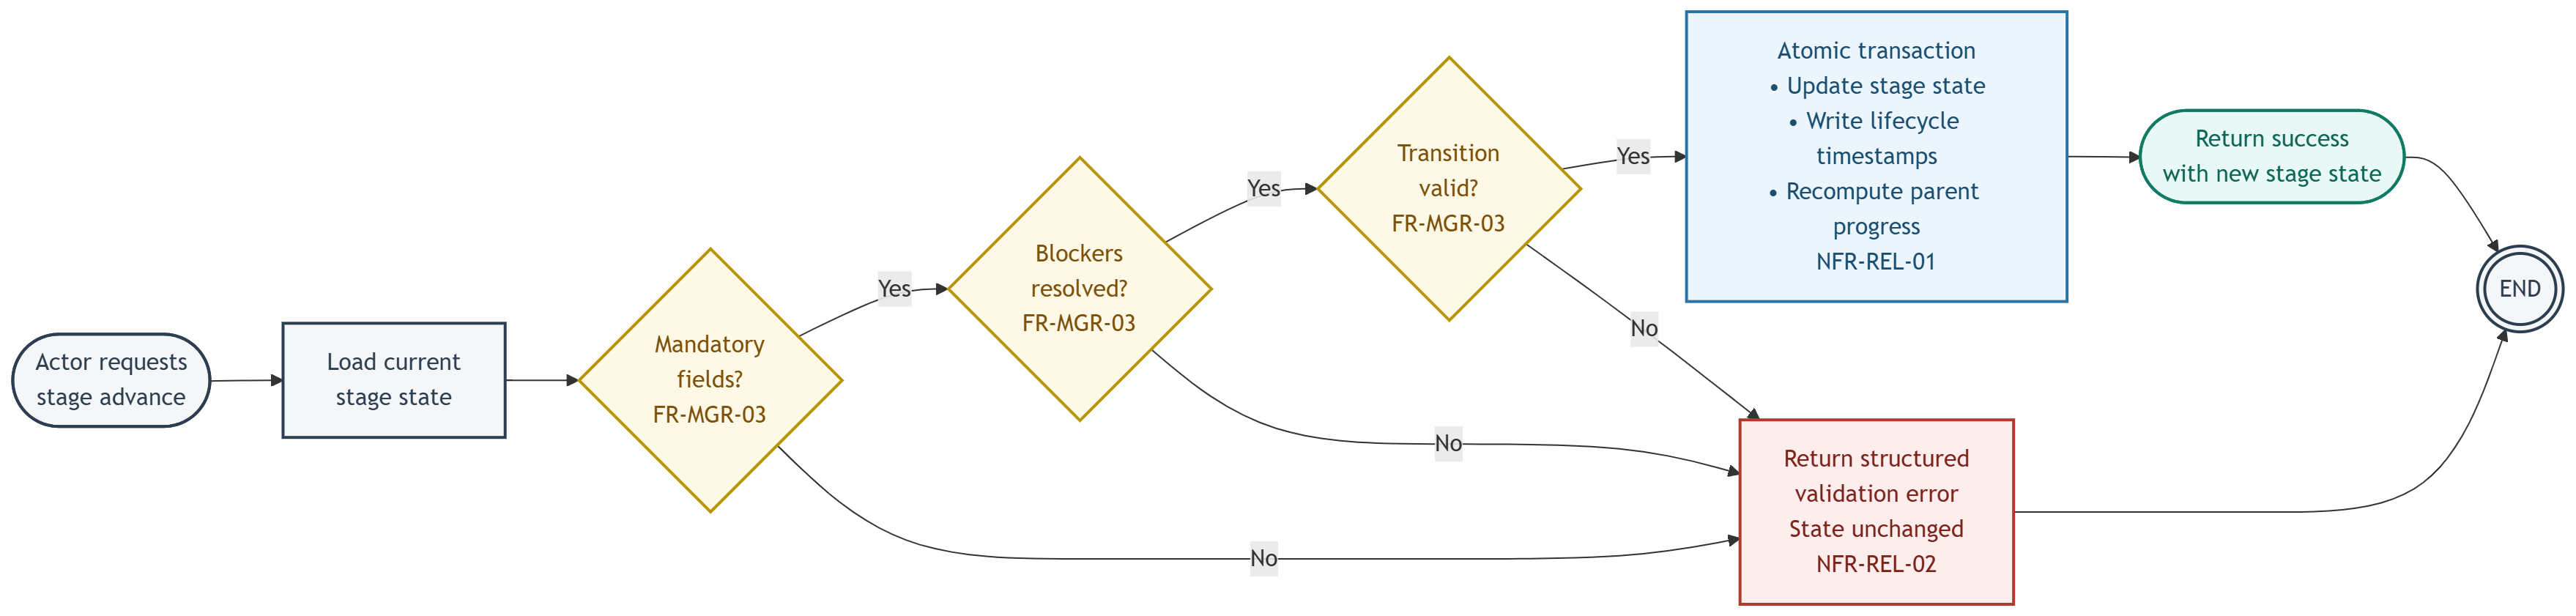
\includegraphics[width=0.85\linewidth,keepaspectratio]{images/fig_3_2_advance_stage.png}%
    }{%
        \fbox{%
            \begin{minipage}[c][6cm][c]{\linewidth}
                \centering
                \textit{[Figure 3.2 placeholder]}
            \end{minipage}%
        }%
    }
    \caption{Activity diagram for \textit{Advance RFQ Stage}}
    \label{fig:activity_advance_stage}
\end{figure}

\subsection{Conversational Flow with the Copilot}
The conversational execution flow diverges structurally from the standard lifecycle workflows of the manager service: a single user interaction (turn) traverses a multi-stage pipeline, heavily relying on deterministic policy evaluations prior to any language-model invocation. This intricate pipeline architecture is detailed conceptually in Chapter~\ref{chap:architecture} and technically in Chapter~\ref{chap:implementation}.

\section{Methodology}\label{sec:methodology}
The methodology governing this project was engineered to mitigate the constraints of a single-developer environment operating asynchronously with academic supervisors and a remote industrial client. The adopted frameworks ensure engineering rigor despite these constraints.

\subsection{Scrumban as the Iteration Framework}
Strict adherence to either Scrum or Kanban paradigms is suboptimal for a single-developer project characterized by asynchronous stakeholder availability. Traditional Scrum ceremonies lack efficacy without a dedicated team, whereas pure Kanban omits the structured demonstration cadence necessary for remote stakeholder alignment. Consequently, this project adopted \textit{Scrumban}, a hybrid framework retaining Scrum's iterative cadence and demonstration discipline, while integrating Kanban's Work-In-Progress (WIP) limits to replace fixed-length sprints. 

The Scrumban board implements a six-state workflow (Figure~\ref{fig:scrumban}): \textit{Backlog (Frozen Scope)}, \textit{Ready}, \textit{In Progress}, \textit{Review and Demo}, \textit{Done}, and \textit{Documented}. Critically, the terminal \textit{Documented} state integrates technical documentation directly into the Definition of Done (DoD). A feature transitions from \textit{Done} only after its technical specification, architectural rationale, and validation evidence are formalized and committed synchronously with the codebase. This rigorous discipline ensures that this report is founded upon artifacts generated during active implementation rather than ex-post reconstruction.

\begin{figure}[H]
    \centering
    \IfFileExists{images/fig_3_3_scrumban.png}{%
        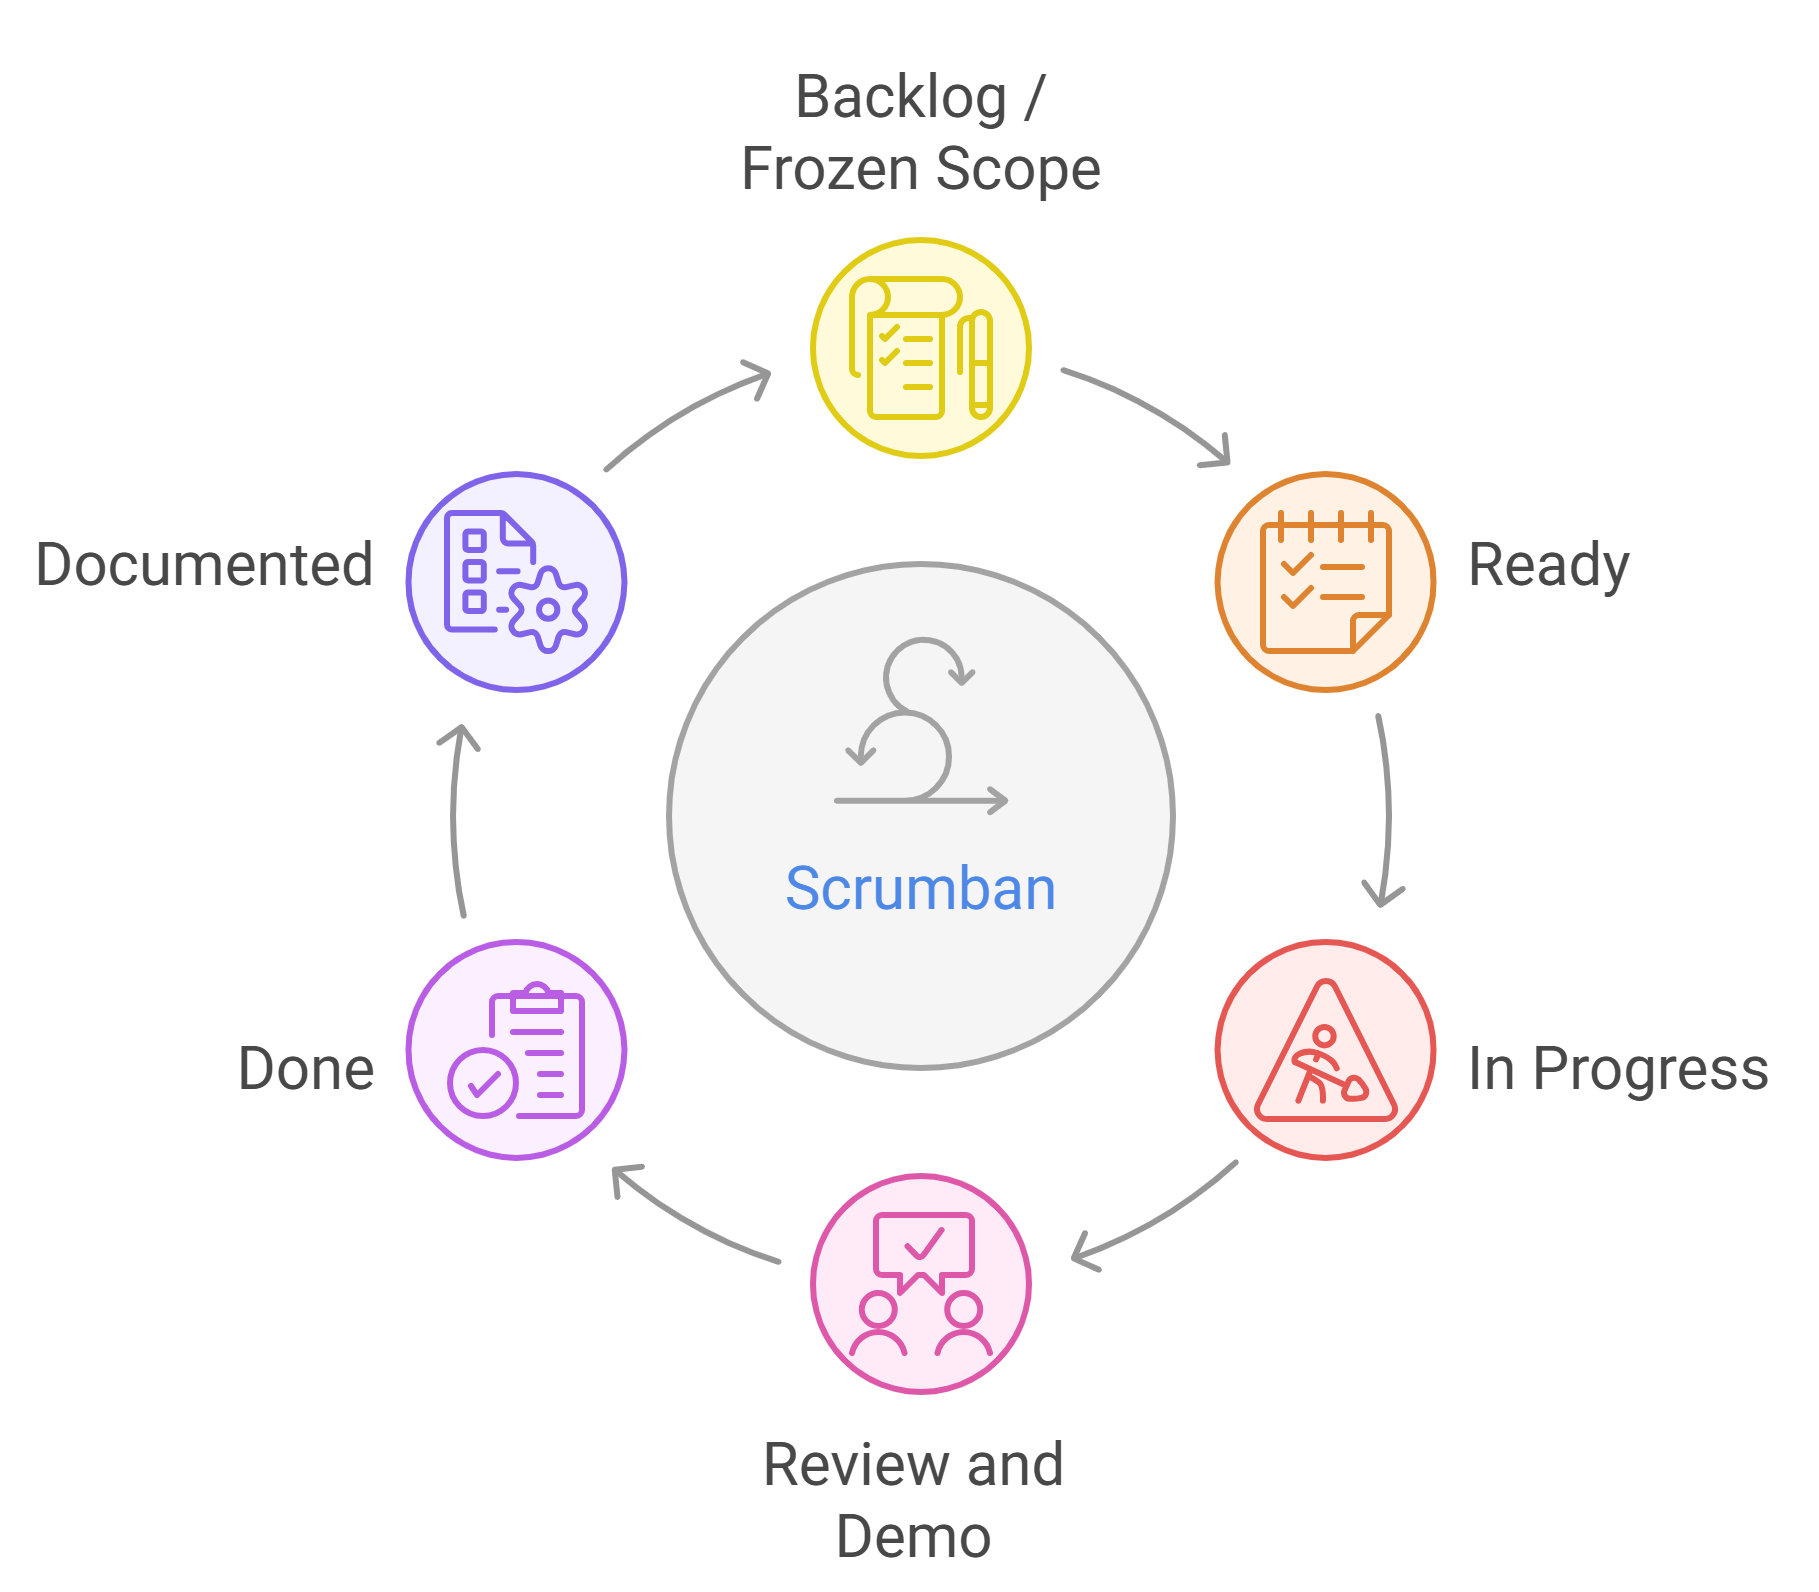
\includegraphics[width=0.85\linewidth,keepaspectratio]{images/fig_3_3_scrumban.png}%
    }{%
        \fbox{%
            \begin{minipage}[c][6cm][c]{\linewidth}
                \centering
                \textit{[Figure 3.3 placeholder]}
            \end{minipage}%
        }%
    }
    \caption{Scrumban six-state workflow board, utilizing \textit{Documented} as the terminal validation column}
    \label{fig:scrumban}
\end{figure}

\subsection{Architectural Decision Records}
Architectural Decision Records (ADRs) adhere to a standardized six-part schema: context, options, decision, justification, consequences, and validation. ADR-H5 (\textit{Dormant Models}) is committed to the manager repository as a fully formalized paradigm; subsequent decisions are systematically documented within Chapter~\ref{chap:architecture}.

\subsection{Project Control Center}
The Scrumban board, decision register, risk register, and stakeholder alignment matrix are centralized within a project Control Center deployed on Notion. This workspace is structured across twelve operational sections governing scope, backlog tracking, architectural decisions, and risk mitigation. The Control Center functioned as the single source of truth for project state throughout the development iteration; data extracted from this centralized repository forms the empirical basis for the tables and artifacts presented in this chapter and throughout the report.

\section*{CONCLUSION}
\addcontentsline{toc}{section}{CONCLUSION}
This chapter has formalized the systemic engineering structure of the project: identifying stakeholders, actors, and access models; delineating twenty-five functional and nineteen non-functional requirements; establishing behavioral use cases; and defining the agile methodology. The subsequent chapter formulates the technical architecture designed to satisfy these rigorous requirements.
